\documentclass[14pt,a4paper]{report}
%\documentclass[master]{disser}
\usepackage{extsizes}% нестандартный 14-ый размер шрифта
\usepackage[left=30mm,right=15mm,top=20mm,bottom=20mm,binding offset=0cm]{geometry} % поля страницы
\usepackage[utf8]{inputenc} % Кодировка текста
\usepackage[T1,T2A]{fontenc} % Кодировка шрифта
\usepackage[english,russian]{babel} % языковая поддержка
\usepackage{indentfirst} % первый параграф раздела начинается с красной строки
\usepackage{misccorr} % исправляет некоторые несоответствия с правилами полиграфии
\usepackage{amssymb,amsmath,amsfonts,latexsym,mathtext} %расширенные наборы математических символов
\usepackage{pdfpages}
\usepackage{listings}
\usepackage{xcolor}
\usepackage{longtable}
\usepackage{lipsum}
\usepackage{biblatex}
\usepackage{filecontents}
\usepackage{enumitem}
\usepackage{hyperref}
\usepackage{caption}
\usepackage{graphicx}
\usepackage[autostyle]{csquotes}
\usepackage{amssymb}
%\usepackage{ntheorem}
\usepackage{amsthm}
%\usepackage{fourier}
\usepackage{nicefrac}
\usepackage{textcomp}

\DeclareMathOperator{\diam}{Diam}

\newtheoremstyle{break}
  {\topsep}{\topsep}%
  {\itshape}{}%
  {\bfseries}{}%
  {\newline}{}%

\theoremstyle{plain}

\newtheorem*{definition1}{Определение}
\newtheorem*{theorem1}{Теорема}
\newtheorem*{lemma1}{Лемма}
\newtheorem*{statement1}{Утверждение}

\newtheorem{definition}{Определение}
\newtheorem{theorem}{Теорема}
\newtheorem{lemma}{Лемма}
\newtheorem{statement}{Утверждение}

\theoremstyle{break}
\newtheorem*{theorem_break1}{Теорема}

\setlist[enumerate]{leftmargin=1cm,topsep=0pt,itemsep=-1ex,partopsep=1ex,parsep=1ex,ref=\arabic{*},label=\arabic{*}.}

\setlength\parindent{1cm}

\linespread{1.3} % полуторный межстрочный интервал

%Нумерация странниц
\usepackage{fancyhdr} % пакет для установки колонтитулов
\pagestyle{fancy} % смена стиля оформления страниц
\fancyhf{} % очистка текущих значений
\fancyhead[LE,RO]{}
\fancyhead[LO,RE]{}
\fancyfoot[CE,CO]{}
\fancyfoot[LE,RO]{}
\fancyhead[C]{\thepage} % установка верхнего колонтитула
\renewcommand{\headrulewidth}{0pt} % убрать разделительную линию

\frenchspacing % везде одинарные пробелы в тексте

\title{SCIENTIFIC WORK} % название документа

\addbibresource{chapters/references.bib}

\begin{document} % начало тела документа

\includepdf[pages=-]{chapters/title.pdf}


\newpage

% \thispagestyle{empty} % неотображает номер страницы %

\begin{center}
\textbf{СОДЕРЖАНИЕ}
\end{center}
\vspace{1.5mm}

\begin{description}

\item{ВВЕДЕНИЕ} \dotfill \pageref{chapters:introduction}

\item{ГЛАВА 1.} РАСКРАСКИ СФЕР \dotfill \pageref{chapters:1}
\begin{enumerate}
\item[1.1] Постановка задачи и известные результаты \dotfill \pageref{chapters:1.1}
\item[1.2] Разбиение на области Вороного \dotfill \pageref{chapters:1.2}
\item[1.3] Задача Томсона \dotfill \pageref{chapters:1.3}
\end{enumerate}

\item{ГЛАВА 2.} ЗАДАЧА ВЫПОЛНИМОСТИ БУЛЕВЫХ ФОРМУЛ И SAT-РЕШАТЕЛИ \dotfill \pageref{chapters:2}
\begin{enumerate}
\item[2.1] Определения \dotfill \pageref{chapters:2.1}
\item[2.2] Алгоритм DPLL \dotfill \pageref{chapters:2.2}
\item[2.3] Алгоритм CDCL \dotfill \pageref{chapters:2.3}
\item[2.4] Детали реализации современных SAT-решателей \dotfill \pageref{chapters:2.4}
\end{enumerate}

\item{ГЛАВА 3.} ВЕРХНИЕ ОЦЕНКИ ХРОМАТИЧЕСКИХ ЧИСЕЛ СФЕР \dotfill \pageref{chapters:3}
\begin{enumerate}
\item[3.1] Численные эксперименты \dotfill \pageref{chapters:3.1}
\item[3.2] Теоретические оценки \dotfill \pageref{chapters:3.2}
\end{enumerate}

\item{ЗАКЛЮЧЕНИЕ} \dotfill \pageref{chapters:conclusions}
\item{СПИСОК ИСПОЛЬЗОВАННЫХ ИСТОЧНИКОВ} \dotfill \pageref{chapters:biblio}

\item{ПРИЛОЖЕНИЕ 1. ДИАПАЗОНЫ ЗНАЧЕНИЙ РАДИУСА ДЛЯ РЕШЕНИЙ ЗАДАЧИ ТОМСОНА} \dotfill \pageref{attachments:1}
\item{ПРИЛОЖЕНИЕ 2. КОДИРОВАНИЕ ЗАДАЧИ РАСКРАСКИ ГРАФА} \dotfill \pageref{attachments:2}
\item{ПРИЛОЖЕНИЕ 3. ВЫЧИСЛЕНИЕ ГРАНИЦ ДИАПАЗОНОВ ЗНАЧЕНИЙ РАДИУСА} \dotfill \pageref{attachments:3}
\item{ПРИЛОЖЕНИЕ 4. ПОСТРОЕНИЕ ДИАГРАММЫ ВОРОНОГО С ИКОСАЭДРАЛЬНОЙ СИММЕТРИЕЙ} \dotfill \pageref{attachments:4}
\item{ПРИЛОЖЕНИЕ 5. ВИЗУАЛИЗАЦИЯ РАСКРАСОК} \dotfill \pageref{attachments:5}

\end{description}


%\pagenumbering{arabic}

\newpage
\begin{center}
\noindent\textbf{ВВЕДЕНИЕ}\label{chapters:introduction}
\vspace{1.5mm}
\end{center}

Целью настоящей дипломной работы является получение конструктивных верхних оценок для хроматического числа двумерной сферы, 
то есть построения таких раскрасок сферы, при которых точки, находящиеся на единичном расстоянии, раскрашены по-разному. 
Это задача примыкает к области классических исследований плотнейших упаковок и редчайших покрытий сфер, находится на стыке
теории графов, комбинаторной геометрии и теории кодирования.
Актуальность данной работы обусловлена отсутствием конструктивных методов получения раскрасок сфер и слабой изученностью рассматриваемой задачи, в отличие от асимптотики хроматических чисел $n$-мерных сфер при $n\to\infty$.

Для достижения поставленной цели необходимо решить следующие задачи:

\begin{enumerate}[leftmargin=1cm,topsep=0pt,itemsep=-1ex,partopsep=1ex,parsep=1ex,label=\arabic{*}.]

\item Cвести задачу о раскраске графа в $m$ цветов к задаче булевой выполнимости.
\item Провести исследование алгоритмов и методов, применяемых при построении современных \textit{SAT}-решателей.
\item Применить \textit{SAT}-решатели для поиска хроматического числа графов и получить корректные раскраски сфер, вычислить диапазоны радиусов.
\item Получить оценки хроматических чисел сфер на основе решений задачи Томсона о минимуме потенциала системы $k$ точечных зарядов на сфере и разбиений на области Вороного.
\item Доказать нижние оценки для хроматических чисел квадратов двойственных графов (триангуляций Делоне).

\end{enumerate}

Рассматриваемая задача тесно связана с классической задачей Нелсона — Эрдёша — Хадвигера о хроматическом числе $\chi(\mathbb{R}^2)$ континуального графа, вершинами которого являются точки плоскости, причем ребрами соединены вершины, находящиеся на единичном евклидовом расстоянии. Иными словами, требуется раскрасить плоскость в конечное число цветов так, чтобы точки, находящиеся на единичном расстоянии, имели разный цвет. Какое наименьшее число цветов для этого потребуется? В настоящее время известно, что $5 \leq \chi(\mathbb{R}^2) \leq 7$. Если вторая оценка тривиальна и основана на раскраске гексагонального замощения (\figurename{ \ref{introduction:fig:plane}}), то оценка снизу была получена Хойле [\ref{bib:Heule2018}] лишь в 2018 году при помощи компьютерных вычислений. 

\begin{figure}[h]
\centering
\captionsetup{justification=centering}
\center{\includegraphics[width=0.4\paperwidth]{chapters/introduction/plane.png}}
\caption{Раскраска плоскости в 7 цветов.}
\label{introduction:fig:plane}
\end{figure}

Аналогичную задачу можно поставить для произвольного метрического пространства. Известно, что 
$6 \leq \chi(\mathbb{R}^3) \leq 15$ [\ref{bib:Nech}, \ref{bib:Coul}], 
получены ряд оценок для $\chi(\mathbb{R}^n)$ при $n \ge 3$, а также асимптотика $\chi(\mathbb{R}^n)$ при $n\to\infty$: 
$(1.239...+o(1))^n\leq \chi(\mathbb{R}^n)\leq (3+o(1))^n$ [\ref{bib:Rai1}, \ref{bib:Larm}].
Также рассматривались хроматические числа рациональных пространств $\mathbb{Q}^n$, многомерных сфер $S^n(r)$, 
множеств вида $\mathbb{R}^2 \times \left[ 0,~\varepsilon \right]^{k}$, ограниченных множеств, точек плоскости с координатами, принадлежащими некоторому квадратичному расширению $\mathbb{Q}$, хроматические числа пространств с запрещенными одноцветными треугольниками. Как правило, полагают, что расстояние между точками множества индуцировано евклидовой метрикой $\mathbb{R}^n$. Основополагающим результатом в данной области является следующая теорема [\ref{bib:BruijnErdos}].


\begin{theorem1}[Эрдеш-де Брейне]
Если $G$ — граф с множеством вершин произвольной мощности, и $\chi(G) = k$. Тогда найдется конечный подграф  $\widetilde{G} \subseteq G$, для которого $\chi(\widetilde{G}) = k$. 
\end{theorem1}

Это означает, что наилучшую из возможных оценок хроматического числа снизу всегда можно обосновать, перебирая подграфы с конечным числом вершин. Препятствием для осуществления такого перебора (даже в случае $\mathbb{R}^2$) является, во-первых, комбинаторный взрыв, а во-вторых, отсутствие методов, позволяющих раскрасить континуальный граф в тех случаях, когда критический подграф (предположительно) найден.

Отдельный класс задач возникает в том случае, если на раскраску накладываются дополнительные ограничения, например, измеримость каждого из множеств, раскрашенных в один из цветов. Еще более жесткое условие — выпуклость компонент связности одноцветных подмножеств, для плоскости — раскраска многоугольных областей. Тогда для раскраски двумерного гладкого многообразия, удовлетворяющего определенным условиям, требуется не менее 7 цветов [\ref{bib:Soifer},\ref{bib:Kronk}].

\newpage
\begin{center}
\noindent\textbf{ГЛАВА 1. РАСКРАСКИ СФЕР}\label{chapters:1}
\vspace{1.5mm}
\end{center}

\vspace{5pt}
\textbf{1.1 Постановка задачи и известные результаты}\label{chapters:1.1}
\vspace{5pt}

Графом называется пара $G=(V,~E)$, где $V$ -- вершины графа, $E \subseteq \{\, (u,v) \mid u,v \in V \,\}$ -- ребра графа. 
Хроматическим числом графа $\chi(G)$ называется минимальное число $k$ такое, что множество вершин $V$ можно разбить (покрасить) на $k$ 
непересекающихся классов $V_1 \sqcup V_1 \sqcup \dots \sqcup V_k = V$ так, что никакое ребро из $E$ не соединяет вершины одного класса. 
В данной работе рассматривается задача о хроматическом числе двумерной сферы 
$S^2(r) = \{\, x \in \mathbb{R}^3 : \|x\| = r \,\}$, сформулированная Полом Эрдёшем в 1981 году [\ref{bib:ErdosGraham}].
Предполагается, что расстояние между точками сферы $x,y \in S^2(r)$ задано евклидовой метрикой в $\mathbb{R}^3$: 
$d(x,y) = \sqrt{\sum_{i=1}^{3}(x_i-y_i)^2}$. Тогда 
$\chi(S^2(r)) = \min \{\, k: S^2(r) = V_1 \sqcup \dots \sqcup V_k , \, x,y \in V_i \Rightarrow \|x - y\| \ne 1 \,\}$. 
Во всех случаях, когда требуются непосредственные вычисления, предполагается, что центр сферы находится в начале координат.

Очевидно, что $\chi(S^2(r))$ зависит от $r$: если $r < \tfrac{1}{2}$, то $\chi(S^2(r))=1$, в то же время 
$S^2\left(\tfrac{1}{2}\right) = 2$ (подходит любая раскраска, в которой диаметрально противоположные точки имеют разный цвет).
При $r > \tfrac{1}{2}$ выполнено $\chi(S^2(r))>2$, так как соответствующий континуальный граф $G(S^2(r); 1)$ содержит нечетный цикл, для раскраски которого необходимы по крайней мере $3$ цвета.
В статье [\ref{bib:Simmons}] Симмонса был получен следующий результат:

\begin{theorem1}[Симмонс, 1976]
$$ \chi\left(S^2\left(\frac{1}{\sqrt{2}}\right)\right)=4, \quad \chi(S^2(r)) \geq 4 \text{ при } r > \frac{1}{\sqrt{3}}. $$
\end{theorem1}

Последнее неравенство было получено вложением в сферу конструкции, аналогичной \enquote{свернутому} веретену Мозера (\figurename{ \ref{chapter1:fig:simmons}}), для раскраски которой необходимо $4$ цвета. 
Отметим, что раскраска сферы $\chi\left(S^2\left(\frac{1}{\sqrt{2}}\right)\right)$ возникает в некой задаче квантовой механики, вследствие чего этот результат был переоткрыт другими авторами. Случай интересен тем, что $d(u,v)=1$ эквивалентно $(u,v)=0$ .
Из неравенства $\chi(\mathbb{R}^3) \leq 15$ следует, что 
$$\forall r>0 \quad \chi(S^2(r)) \leq 15.$$

\begin{figure}[h]
\centering
\captionsetup{justification=centering}
\begin{minipage}[h]{0.5\linewidth}
\center{\includegraphics[width=0.4\paperwidth]{chapters/chapter1/simmons2.png}}
\end{minipage}\hfill
\begin{minipage}[h]{0.5\linewidth}
\center{\includegraphics[width=0.4\paperwidth]{chapters/chapter1/simmons.png}}
\end{minipage}\hfill
\caption{К теореме Симмонса [\ref{bib:Simmons}].}
\label{chapter1:fig:simmons}
\end{figure}

В дополнение к предыдущим рассмотрим некоторые асимптотические оценки. 
В 1983 году  Л. Ловас доказал, что  $\chi(S^{n-1}(r)) \geq n$. В статье [\ref{bib:RaiSphere}] А.М. Райгородским показал, что хроматическое число сферы растет экспоненциально при росте размерности для всех $r > \frac{1}{2}$.

\begin{theorem1}

$$\text{Если } r \in (\frac{1}{2}, \frac{1}{\sqrt{2}}], \text{ то } 
\chi(S^{n-1}(r)) \geq \left(2(\frac{1}{8r^2})^{\frac{1}{8r^2}}(1-\frac{1}{8r^2})^{1-\frac{1}{8r^2}}+o(1)\right)^n.$$ 

$$\text{Если } r \geq \frac{1}{\sqrt{2}}, \text{ то } 
\chi(S^{n-1}(r)) \geq \left(2(\frac{1}{4})^{\frac{1}{4}}(\frac{3}{4})^{\frac{3}{4}}+o(1)\right)^n.$$

\end{theorem1}
В работе [\ref{bib:Kostina}] О. Костина доказала усиленный вариант предыдудщей теоремы.

\begin{theorem1}
Пусть $r > \tfrac{1}{2}$ и $b_1, b_{-1}$ таковы, что $b_1 + b_{-1} \in (0,1]$ и $b_1 < b_{-1}$.
Пусть $k_1=[b_1n]$ и $k_{-1}=[b_{-1}n]$. Положим

$$p_0(r,b_1,b_{-1},n) = \frac{(k_1 + k_{-1})n - (k_1 + k_{-1})^2}{2nr^2}$$
Пусть $p(r,b_1,b_{-1},n)$ -- минимальное простое число, строго большее, чем $p_0$. 
Если при данных $r,b_1,b_{-1},n$ выполнено $k_1 + k_{-1} - 2p < -2k_{-1}$, то

$$\chi(S^{n-1}(r)) \geq 
\frac{\binom{n}{k_1}\binom{n-k_1}{k_{-1}}}
{\sum\limits_{(m_1,m_2) \, \in \, \mathcal{A}} \binom{n}{m_1} \binom{n-m_1}{m_2}}$$
где $\mathcal{A} = \{ (m_1,m_2): m_1,m_2 \in \mathbb{N} \cup \{ 0 \}, m_1+m_2 \leq n, m_1+2m_2 \leq p-1 \}$.

\end{theorem1}

Очевидно, что $\chi(S^{n-1}(r)) \leq \chi(\mathbb{R}^n) \leq (3+o(1))^n$, т.к. $S^{n-1}(r)$ лежит в $\mathbb{R}^n$. В общем случае лучших верхних оценок нет. Однако К.А. Роджерс [\ref{bib:Rogers}] получил более точную оценку в случае $r < \frac{3}{2}$.

\begin{theorem1}
$$\text{Если } r < \frac{3}{2}, \text{ то } \chi(S^{n-1}(r)) \leq (2r+o(1))^n.$$
\end{theorem1}

В работе [\ref{bib:Pros}] Р. Просановым получена следующая верхняя оценка хроматического числа сферы:

\begin{theorem1}
$\chi(S_r^{n-1}) \leq (x(r)+o(1))^n$, где
$$ x(r) = 
\begin{cases}
\sqrt{5-\frac{2}{r}+4\sqrt{1-\frac{5r^2-1}{4r^4}}},& \quad r > \frac{\sqrt{5}}{2} \\ 
2r,& \quad \frac{1}{2} < r \leq  \frac{\sqrt{5}}{2}
\end{cases}.$$
\end{theorem1}

Так как шестиугольники в раскраске плоскости (\figurename{ \ref{introduction:fig:plane}}) допускают небольшие деформации, кажется, что \enquote{почти плоский} участок сферы большого радиуса может быть раскрашен в $7$ цветов. Напрашивается заключение, что при достаточно большом $r$ в $7$ цветов может быть покрашена вся сфера, но на самом деле, как будет показано далее, аналогичных раскрасок всей сферы не существует. Тем не менее этот подход позволяет построить корректные 
раскраски сфер для некоторых диапазонов радиусов и получить на их основе верхние оценки для $\chi(S^2(r))$.

\vspace{5pt}
\textbf{1.2 Разбиение на области Вороного}\label{chapters:1.2}
\vspace{5pt}

Рассматриваются раскраски сферы $S^2(r)$ в $k$ цветов. 
Пусть $c(x)$ -- цвет точки $x$, а $C_i$ -- множество точек, раскрашенных в $i$-й цвет, $\bigcup\limits_{i=1}^{k} C_i = S^2(r)$. 
Требуется выполнить условие:

\begin{equation}\label{chapter1:propercoloring}
\forall \, x,y \in S^2(r), \, \|x - y\|=1 \Rightarrow c(x) \ne c(y)
\end{equation}

В данной работе в качестве таких одноцветных областей $C_i$ предлагается 
рассматривать выпуклые сферические многоугольники, построенные как области Ворон\textbf{о}го для некоторого набора точек.
Если задан набор точек (сайтов, генераторов) $x_1, x_2, \dots , x_m \in S^2(r)$, то диаграммой Вороного называется разбиение
$S^2(r)= \bigcup\limits_{i=1}^m V_i$, где $V_i$ - ячейки Вороного:
$$V_i = \{y \in S^2(r) \, : \quad \|y - x_j\| \geq \|y - x_i\|, \quad 1 \leq j \leq n, \, j \neq i \}.$$

Поскольку мы будем красить каждую область Вороного в один цвет, потребуем $\diam V_i < 1$, и, 
дополнительно, $\diam (V_i \bigcup V_j) > 1$, 
то есть мы не рассматриваем разбиение на области, которые могут быть объединены с соседними. 

В зависимости от контекста будем называть диаграммой Вороного как разбиение на ячейки, так и граф из вершин и ребер, составляющих эти ячейки. Такие мозайки названы в честь русского математика Георгия Вороного, который описал общий $n$-мерный случай в 1908 году,
являются фундаментальным инструментом вычислительной геометрии, широко используются в компьютерной графике, $3D$-моделировании, картографии, геофизике, химии, биологии. 
Для построения разбиений Вороного предложен ряд эффективных ($O(n\log{}n)$) алгоритмов и их компьютерных реализаций: 
\textit{CGAL}, \textit{TRIPACK}, \textit{STRIPACK}, \textit{Triangle}, \textit{QHull}, 
[\ref{bib:Larrea}], последний из которых является модификацией алгоритма Кларксона-Шора [\ref{bib:Barber}] и использовался в данной работе.

Мозайке Вороного однозначно соответствует граф триангуляции Делоне (состоящий из непересекающихся отрезков, соединяющий заданный набор точек так, что при построении плоскости через три точки, которые образуют треугольник, все остальные точки лежат не выше этой плоскости), который можно построить за $O(n)$:

\begin{theorem1}
Если соединить все сайты, соответствующие смежным ячейкам диаграммы Вороного, получится (двойственный) граф триангуляция Делоне для этого множества точек.
\end{theorem1}

\begin{figure}[h]
\centering
\captionsetup{justification=centering}
\center{\includegraphics[width=0.3\paperwidth]{chapters/chapter1/triang-example.png}}
\caption{Диаграмма Вороного и двойственная триангуляция.}
\label{chapter1:fig:triangexample}
\end{figure}

На \figurename{ \ref{chapter1:fig:triangexample}} приведен пример мозайки (синим) и двойственного графа.
Отметим, что для заданного набора точек сферическая триангуляция Делоне всегда существует, причём для каждого набора точек, в котором никакие четыре не лежат на одной окружности, она единственна.
Пусть задана набор точек и диаграмма Вороного. Обозначим как $\mathcal{G}$ граф триангуляции Делоне, двойственной к данной диаграмме. Предположим, что каждая из областей Вороного покрашена в некоторый цвет, и эта раскраска удовлетворяет условию 
(\ref{chapter1:propercoloring}). Раскрасим вершины $\mathcal{G}$ в цвета соответствующих областей. Тогда справедливы следующие утверждения.

\begin{statement}\label{chapter1:statement1}
Цвета смежных вершин $\mathcal{G}$ различны. 
\end{statement}

\begin{proof}
Предположим, что это неверно. Тогда объединение двух одноцветных областей имеет диаметр больше $1$, а поскольку это множество связно, то оно содержит и две одноцветные точки на единичном расстоянии, что противореит (\ref{chapter1:propercoloring}).
\end{proof}
 
\begin{statement}\label{chapter1:statement2}
Цвета вершин $\mathcal{G}$, находящихся на расстоянии $2$ (в смысле длины кратчайшего пути в графе), различны. 
\end{statement}

\begin{proof}
Поскольку диаметр любой области не превосходит единицы, расстояние между областями, имеющими общего соседа, меньше единицы,
значит найдется отрезок длины $1$, лежаший концами в этих областях. Следовательно, они должны иметь разные цвета.
\end{proof}

Пусть $\mathcal{G}^2$ -- граф, в котором множество вершин совпадает с множеством вершин $\mathcal{G}$, 
а к ребрам из $\mathcal{G}$  добавлены ребра, соединяющие вершины, 
которые в графе $\mathcal{G}$ находились на расстоянии $2$:
$$E(\mathcal{G}^2) = \{ (u,v): \, (u,v) \in E(\mathcal{G}) \lor \exists \, w: \, (u,w),\,(w,v) \in E(\mathcal{G}) \}.$$
Тогда из построения $\mathcal{G}^2$ и утверждений 
\ref{chapter1:statement1} и \ref{chapter1:statement2} вытекает следующее.

\begin{statement}
Для существования правильной раскраски диаграммы Вороного в $k$ цветов необходимо, чтобы $\chi(\mathcal{G}^2) \leq k$.
\end{statement}

Если расстояние между $V_i$ и $V_j$, $i \neq j$ меньше единицы тогда и только тогда, 
когда соответствующие вершины смежны в $\mathcal{G}^2$, то последнее утверждение является необходимым и достаточным условием существования правильной раскраски сферы. Учитывая предыдещие построения и рассуждения, 
раскраску сферы в $k$ цветов получить из \enquote{подходящего} набора точек следующим образом: 
построить для них диаграмму Вороного, двойственный граф триангуляции $\mathcal{G}$, его квадрат $\mathcal{G}^2$, 
найти $k = \chi(\mathcal{G}^2)$, проверить выполнение всех необходимых условий и вычислить набор радиусов, 
при которых они выполняются. 
Основой для выбора точек-генераторов $\{ x_i \}$, соответствующих решениям задачи Томсона, стала следующая гипотеза.

\begin{hypothesis}
При некоторых $N$ локальный минимум в задаче Томсона индуцирует разбиение сферы на области Вороного, для которого минимум расстояния между областями, находящимися на расстоянии $2$ в двойственном графе, строго больше максимума диаметров областей разбиения.
\end{hypothesis}

Данная гипотеза была подтверждена компьютерными вычислениями.
Если $d0$ -- максимальный из диаметров областей $V_i$, $d1$ -- минимальное из расстояний между областями на расстоянии $2$, то при выполнении всех остальных ограничений диапазон радиусов можно получить как 
\begin{equation}\label{chapter1:radiuseq}
\left( \nicefrac{1}{d1}, \, \nicefrac{1}{d0} \right), \text{ где } \nicefrac{d1}{d0} < 1
\end{equation}

Поиск хроматического числа графа является сам по себе сложной задачей. Для ее решения в данной работе использовались 
\textit{SAT}-решатели, которым посвящена вторая глава. Алгоритм поиска $\chi(G)$ вытекает из следующего утверждения.

\begin{statement1}\label{chapter1:formula}
Задача раскраски графа $G=(V,E)$ в $n$ цветов эквивалентна задаче булевой выполнимости формулы
$$F(G,n) = 
\bigwedge\limits_{v \in \textit{V}} 
\left( c_v^1 \vee \dots \vee c_v^n \right) 
\wedge 
\bigwedge\limits_{v \in \textit{V}, \, i < j \leq n } 
\left( \bar{c_v^i\vphantom{c_v^j}} \vee \bar{c_v^j} \right) 
\wedge 
\bigwedge\limits_{(v,w) \in \textit{E}, \, i \leq n} 
\left( \bar{c_v^i} \vee \bar{c_w^i} \right) \,$$
где переменная $c_v^i$ равна $1$ тогда и только тогда, когда вершина $v$ покрашена в цвет $i$.
\end{statement1}

\vspace{5pt}
\textbf{1.3 Задача Томсона}\label{chapters:1.3}
\vspace{5pt}

Множества точек $\{ x_i \}$, \enquote{равномерно} распределенных на поверхности сферы, возникают как решения трудоемких задач многомерной оптимизации: задачи Томсона (о минимизации потенциала распределения точечных зарядов на сфере) и задачи о сферических кодах (максимизация минимального из попарных расстояний). 

Первая из задач сформулирована Дж. Дж. Томсоном в 1904 году [\ref{bib:Thomson}] при изучении \enquote{пудинговой} модели атома. 
Необходимо определить минимальную конфигурацию полной потенциальной энергии системы $N$ электронов, ограниченных поверхностью единичной сферы, которые отталкиваются друг от друга силой, определяемой Законом Кулона:

\begin{equation}\label{chapter1:thomson}
V(x_1, \dots, x_N) = \sum\limits_{i,j} \frac{1}{ \|x_i-x_j\| } \to \min\limits_{(x_1, \dots, x_N)}
\end{equation}

Cпустя век после постановки задача Томсона в трехмерном пространстве решена только для случаев 
$N = 2, 3, 4, 5, 6, 12$. 
При $N = 1$ решение тривиально. 
Два электрона располагаются в диаметрально противоположных точках.
Три электрона располагаются на большой окружности сферы в вершинах правильного треугольника.
Четыре электрона располагаются в вершинах правильного тетраэдра.
Для $N = 5$ в 2010 году было получено строгое компьютерное решение с электронами, находящимися в вершинах треугольной дипирамиды.
При $N = 6$ электроны находятся в вершинах правильного октаэдра.
При $N = 12$ электроны находятся в вершинах правильного икосаэдра.
При других $N$ экстремальность какой-либо конфигурации не доказана, 
однако для наших целей подходят и субоптимальные решения. Рассмотрим несколько алгоритмов их получения.

\textbf{Метод решетки} [\ref{bib:Altschuler}] позволяет получить расположение точек при $N = 10(m^2 + n^2 + mn) + 2$, 
где $m,n$ -- целые числа, $N < 5000$. 
Пусть $\zeta = e^{\frac{i\pi}{3}}$, $\Delta$ - 
равносторонний треугольник с вершинами $0, m + \zeta n, \zeta m + \zeta^2 n$. Пересечение решетки $\Lambda$ с базисом $1, \zeta$ 
и треугольника $\Delta$ -- конечное множество точек $\Delta$, которое отображается на грань вписанного в сферу икосаэдра. 
Остальные грани икосаэдра заполняются поворотом на $180^{\circ}$ относительно центра общего ребра соседних треугольников. 
Далее все полученные вершины радиально проецируются на поверхность сферы, после чего функционал суммарной энергии 
(\ref{chapter1:thomson}) оптимизируется методом сопряженных градиентов. 
$\upsilon_1(N)$ -- количество целых чисел $l \le N$, для которых описанный алгоритм позволяет разместить электроны 
на поверхности сферы (существует решение соответствующего диофантова уровнения) можно грубо оценить как
$\upsilon_1(N) = 0.018N + 2.1\sqrt{N} + o(\sqrt{N})$.
На \figurename{ \ref{chapter1:fig:thomson}} приведен пример расположений зарядов для случаев $N=132$ (слева) и $N=1032$, полученных таким способом.

\begin{figure}[h]
\centering
\captionsetup{justification=centering}
\begin{minipage}[h]{0.5\linewidth}
\center{\includegraphics[width=0.35\paperwidth]{chapters/chapter1/thomson1.png}}
\end{minipage}\hfill
\begin{minipage}[h]{0.5\linewidth}
\center{\includegraphics[width=0.35\paperwidth]{chapters/chapter1/thomson2.png}}
\end{minipage}\hfill
\caption{Субоптимальные решения задачи Томсона [\ref{bib:Altschuler}].}
\label{chapter1:fig:thomson}
\end{figure}

\textbf{Метод сечения икосаэдра} [\ref{bib:Katanforoush}] позволяет получить расположения лишь 
для $\upsilon_2(N) \simeq c\log{}N$ точек. 
Пусть $ABC$ -- треугольник, и $a,\,b,\,c$ -- середины его сторон $BC,\,CA,\,AB$. 
Тогда треугольник $abc$ разбивает $ABC$ на четыре треугольника (2-разрез). 
Такую операцию можно проделать для всех $20$ граней икосаэдра, 
получив триангуляцию из $80$ граней, $120$ ребер и $42$ вершин, радиальная проекция которой на сферу дает нужный результат. 
Аналогично строится $m$-разрез: каждая сторона треугольника делится на $m$ сегментов, порождая $m^2$ новых треугольников.
Эту операцию можно повторять итеративно, получая все более \enquote{мелкие} разбиения. 

Оба этих метода обладают полезным свойством. Назовем \textit{дефектом} вершины $\upsilon \in V(G)$ 
число $\delta(\upsilon) = 6 - deg(\upsilon)$. 
Тогда для графа триангуляции сферы $G$, построенного методом решетки или методом сечения икосаэдра выполнено 
\begin{equation}\label{chapter1:eq:defect}
\sum\limits_{\upsilon_i \in V(G)} \delta(\upsilon_i) = 12
\end{equation}
Это равенство следует из построений и знаменитой формулы Эйлера для планарных графов: 
$v - e + f = 2$.
В частности, граф $G$ может содержать $12$ вершин степени $5$ и сколь угодно большое число вершин степени $6$. 

Решения, обладающие икосаэдральной симметрией, ($I$ в нотации Шeнфлиса) представляют особый теоретический интерес.
Их можно параметризовать парой натуральных чисел $p,q$ , где $p$ и $q$ -- длины сторон параллелограмма на треугольной сетке, 
противоположные (острые) углы которого расположены в ближайших друг к другу вершинах степени $5$. 
Для графа при $N=132$ (\figurename{ \ref{chapter1:fig:thomson}}) $p=1,q=3$.
Cоответствующий граф будем обозначать $T(p,q)$. 
Некоторые теоретические оценки хроматических чисел для графов такого типа доказаны в третьей главе.

Для численных экспериментов в данной работе были использованы наилучшие 
известные на данный момент конфигурации зарядов для различных $N$ ($12 \le N \le 400$), опубликованные 
в открытой коллекции решений различных оптимизационных задач Кембриджского университета
\textit{The Cambridge Cluster Database} [\ref{bib:Wales}]. 
Они получены различными способами, которые сводятся к выбору \enquote{хорошего} начального расположения
и дальнейшей оптимизации: 
используют градиентные методы, метод Монте-Карло, алгоритм имитации отжига, 
генетические алгоритмы, их комбинации и модификации [\ref{bib:Bondarenko}].

Отметим, что в ходе предварительных исследований рассматривалась идея улучшения имеющихся решений задачи Томсона
с тем, чтобы расширить интервалы ридиусов (\ref{chapter1:radiuseq}), которые \enquote{покрывают} раскраски, 
построенные из этих решений. Однако ее реализация связана с оптимизацией сложно устроенных, 
недифференцируемых функций и осталась за рамками данной работы.



\newpage
\begin{center}
\noindent\textbf{ГЛАВА 2. ЗАДАЧА ВЫПОЛНИМОСТИ БУЛЕВЫХ ФОРМУЛ И SAT-РЕШАТЕЛИ}\label{chapters:2}
\vspace{1.5mm}
\end{center}

\vspace{5pt}
\textbf{2.1. Определения}\label{chapters:2.1}
\vspace{5pt}

Конъюнктивной нормальной формой (КНФ) называются булева формула вида 
$\Phi_m \left( x_1, x_2, \dots, x_m \right) = D_1 \land D_2 \land \dots \land D_k$,
где каждый дизъюнкт $D_j=t_{j,1} \lor t_{j,2} \lor \dots \lor t_{j,n_j}$, 
и все литералы $t_{j,i}$ – либо переменные, либо их отрицания,
причем переменная может встречаться в дизъюнкте не более одного раза. 
Задача выполнимости КНФ (\textit{ВЫП}, \textit{SAT}) заключается в следующем: для входной формулы $\Phi_m$ указанного вида 
необходимо определить, существует ли набор значений переменных $\left( \alpha_1, \alpha_2, \dots, \alpha_m \right)$ такой,
что $\Phi_m \left( \alpha_1, \alpha_2, \dots, \alpha_m \right) = 1$, выполнима ли $\Phi_m$? 
При этом исследователя часто интересует не только ответ \enquote{да} или \enquote{нет}, но и сам выполняющий набор переменных или доказательство его отсутствия.

Факт принадлежности задачи \textit{ВЫП} к классу $\mathcal{NP}$ является тривиальным. Более содержательное утверждение, 
знаменитая теорема Кука-Левина, открывшее важность этой задачи для теории сложности вычислений, 
а впоследствии и для практических приложений, доказал в 1971 году Стивен Кук (тот же результат независимо получило советский математик Леонид Левин). В своей работе [1] он впервые ввел понятие $\mathcal{NP}$-полной задачи и доказал $\mathcal{NP}$-полноту 
задачи выполнимости КНФ, что сделало ее первой известной $\mathcal{NP}$-полной задачей. 
Идея доказательства состоит в построении формулы, которая выполнима тогда и только тогда, когда соответствующая 
недетерминированная машина Тьюринга, решающая выбранную задачу за полиномиальное время, останавливается с положительным ответом.

Этот результат позволил доказать $\mathcal{NP}$-полноту множества других задач путем полиномиального сведения к ним задачи выполнимости КНФ, что стало стандартным способом доказательства $\mathcal{NP}$-полноты. 
Так, в своей работе [2] 1972 года Ричард Карп доказал $\mathcal{NP}$-полноту $21$ задачи (ныне известных как «список Карпа»), 
среди которых: задача о клике, задача о выполнимости булевых формул с тремя литералами (\textit{3-SAT}, 
для которой известен рандомизированный алгоритм ($\mathcal{PPSZ}$) со сложностью $\mathcal{O} \left( 1.32216n \right)$), 
задача о раскраске графа и другие.

Вокруг исследования задачи выполнимости, ее приложений и обобщений сформировалось 
международное научное сообщество \enquote{\textit{SAT Association}}, проводится ежегодная конференция 
\enquote{\textit{International Conference on Theory and Applications of Satisfiability Testing}}, 
публикуется тематический рецензируемый журнал \enquote{\textit{Jour\-nal on Satisfiability, Boolean Modeling and Computation, JSAT}}.
Среди перспективных направлений научных исслендований можно отметить изучение задач 
\textit{CSP} (задача удовлетворения ограничений), 
\textit{MAX-SAT} (задача поиска максимального количества выполнимых дизъюнктов), 
\textit{\#SAT} и \textit{ALL-SAT} (подсчет количества выполняющих наборов и их поиск), 
\textit{SMT} (задача выполнимости формул в теориях), 
\textit{QBF} (задача о булевой формуле с кванторной приставкой), 
а также конструирование приближенных ($\mathcal{PTAS}$) и рандомизированных алгоритмов.

Пока вопрос о равенстве классов $\mathcal{P}$ и $\mathcal{NP}$ остается открытым, $\mathcal{NP}$-полнота задачи \textit{SAT} свидетельствует о том, что она является вычислительно сложной и у нас нет эффективных детерминированных алгоритмов, позволяющих в общем случае решать ее за разумное время. С другой стороны, ряд важных прикладных задач естественным образом (например, с помощью преобразования Цейтина) сводится к \textit{SAT} и ее обобщениям: задачи из области автоматизации проектирования (\textit{EDA}), логического синтеза, автоматического доказательства теорем, криптографии, биоинформатики, проверки моделей, формальной верификации программ и автоматического конструирования тестовых покрытий, планирования, построения расписаний.

Интерес исследователей, практическая необходимость, развитие вычислительной техники и новые теоретически результаты привели к созданию ряда подходов (и программных пакетов на их основе – \textit{SAT}-решателей), позволяющих во многих случаях эффективно решать задачу выполнимости. 
Все они так или иначе используют модификации метода направленного перебора и в худшем случае имеют экспоненциальную сложность. Их можно условно разделить на несколько семейств по принципу организации перебора:

\begin{enumerate}[label=\arabic{*}.]

\item
Алгоритмы, основанные на поиске с возвратом, из которых наиболее удачным оказался \textit{DPLL} [4] и его улучшенный вариант: \textit{CDCL} [5] и другие подходы, основанные на методе резолюций.

\item
Вариации генетических алгоритмов, например, \textit{GASAT} [6].

\item
Подходы, основанные на применении машинного и глубокого обучения, например, \textit{NeuroSAT} [7], который рассматривает задачу выполнимости как задачу классификации и использует для ее решения рекуррентную нейронную сеть.

\item
Методы стохастического локального поиска [14], например, \textit{WalkSAT}, базовая идея которого заключается в итеративном выборе по некоторому правилу ложного дизъюнкта и \enquote{переворачивании} одного из входящих в него литералов.

\item
Алгоритмы символьных вычислений, основанные на преобразовании бинарной диаграммы решений и ее обобщениях [17].

\item
Алгоритмы, основанные на построении набора правил вывода и пошаговом преобразовании формулы в эквивыполнимую [17].

\end{enumerate}


Современные \textit{SAT}-решатели представляют собой многоуровневые комбинации из нескольких подходов, дополненные различного рода эвристиками (например, случайные рестарты), оптимизациями, преобразованиями формулы [19] (например, исключение переменных методом резолюций или с помощью модифицированной процедуры Фурье-Моцкина) с десятками настраиваемых параметров. Объединение различных техник и тонкая настройка параметров позволяют эффективно решать задачи с тысячами переменных и десятками тысяч дизъюнктов. Отдельного внимания заслуживают детали реализации указанных алгоритмов. Так, мемоизация и специализированные структуры данных могут ускорить выполнение некоторых операций в разы. Другие важные аспекты – возможность инкрементального применения, масштабируемость, эффективное распараллеливание, которое может достигаться несколькими способами: портфельный метод (одновременный запуск нескольких экземпляров решателя); метод \enquote{разделяй и властвуй}, основанный на разбиении формулы на независимые подформулы; параллельный локальный поиск.

Успешность современных алгоритмов при решений индустриальных задач во многом объясняется тем, что они в общем случае имеют регулярную структуру взаимосвязей между переменными. На \figurename{ \ref{chapter1:fig:satgraph}} приведены визуализации индустриальной и случайно сгенерированной задач, полученные методом Clauset-Newman-Moore [24].

\begin{figure}[h]
\centering
\captionsetup{justification=centering}
\center{\includegraphics[width=0.7\paperwidth]{chapters/chapter2/sat-graph.png}}
\caption{Сетевая структура индустриальной (слева) и случайно сгенерированной (справа) формул.}
\label{chapter1:fig:satgraph}
\end{figure}

В качестве примера удачной реализации стратегии \enquote{разделяй и властвуй} можно привести проект построения распределенного \textit{SAT}-решателя \textit{SAT@home} [10], выполненного на платформе для GRID-вычислений \textit{BOINC}, реализованный лабораторией Дискретного анализа и прикладной логики Института динамики систем и теории управления СО РАН, позволивший, в числе прочего, найти несколько ортогональных пар диагональных латинских квадратов порядка $10$.

Не все алгоиртмы являются полными в том смысле, что не гарантируют при любом входе завершиться с корректным ответом. Часто отсутствие полноты становится платой за введение дополнитальных эвристик, которые могут значительно ускорить решение задач некоторого класса. 
Многие реализации алгоритма \textit{CDCL} в случае невыполнимости КНФ позволяют построить \enquote{сертификат невыполнимости} в одном из общепринятых форматов (\textit{TraceCheck}, \textit{DRUP} [8]), которое можно верифицировать специальной утилитой, человеку это сделать обычно не под силу. 
Так, группе ученых во главе с Марином Хойле удалось с помощью \textit{SAT}-решателя и суперкомпьютера \textit{Stampede} ($800$ ядер) построить доказательство в формате \textit{DRAT} отсутствия такой двухцветной раскраски множества $\{1, \dots, 7825\}$, при которой ни одна пифагорова тройка из этого множества не является одноцветной (булева проблема пифагоровых троек) [9]. Размер файла с доказательством достиг $200$ терабайт. Такой метод доказательства утверждений используется все чаще, хотя и не приветствуется математическим сообществом.

\begin{figure}[h]
\centering
\captionsetup{justification=centering}
\center{\includegraphics{chapters/chapter2/sat-competition.png}}
\caption{Результаты The International SAT Competition 2009 года.}
\label{chapter1:fig:satcomp}
\end{figure}

На протяжении двух десятков лет проводятся международные состязания по решению задачи \textit{SAT} [11, 12], на которых участники соревнуются в скорости решения специально подобранных задач, записанных в стандартном формате \textit{DIMACS}, при различных условиях (последовательные, параллельные вычисления) и ограничениях. Построение коротких и \enquote{сложных} конкурсных задач, а также формализация свойств формулы, которые делают ее сложной для \enquote{SAT}-решателя – отдельная интересная проблема. Результаты соревнования 
(\figurename{ \ref{chapter1:fig:satcomp}}) публикуются на сайте \url{http://www.satcompetition.org/}. Победителями этого соревнования в разные годы становились \textit{MiniSAT}, \textit{Glucose}, \textit{Lingeling}, \textit{CryptoMiniSat}, \textit{YalSAT}, \textit{MapleSAT}, \textit{abcdSAT}, \textit{RISS}. Все эти проекты имеют открытый исходный код и доступны для свободного использования. Группа ученых из Университета Британской Колумбии поддерживает коллекцию \textit{SAT}-задач различного уровня сложности, известную как бенчмарк \textit{SATLIB} [13]. На протяжении многих лет наилучшие результаты на таких соревнованиях, а также и при решении практических задач, показывают алгоритмы, базирующиеся на идее \textit{CDCL}, о который и пойдет речь далее в этой главе.

\vspace{5pt}
\textbf{2.2. Алгоритм DPLL}\label{chapters:2.2}
\vspace{5pt}

Алгоритма \textit{DPLL} [4] – это полный и высокоэффективный алгоритм решения задачи выполнимости, основанный на классическом алгоритме решения задач комбинаторной оптимизации: поиск в глубину с возвратом. Он назван в честь своих авторов: Дэвиса, Патнема, Логемана, Лавленда, впервые опубликован в 1962 году и является усовершенствованной версией \textit{DP}, предыдущего алгоритма Дэвиса и Патнема, основанного на методу резолюций.

Далее введем несколько общепринятых в литературе обозначений. 
Поскольку порядок элементов не важен, здесь и далее формулу $\Phi$ удобно представлять как множество дизъюнктов $\{ D_1, \dots, D_k \}$, 
каждый из которых является множеством литералов $\{ t_{j,1}, \dots ,t_{j,n_j} \}$ над переменными из множества $X$. Если множество дизъюнктов пусто, формула считается тривиально выполнимой, если один из дизъюнктов пуст - не выполнимой.
В контексте алгоритмов поиска выполняющих наборов каждая переменная $x \in  X$ может находиться в разных состояниях. Переменной может быть присвоено значение $\nu(x)$, $\nu: X \mapsto \{ 0, 1, ?\}$, где знаком \enquote{$?$} обозначается, что значение переменной не определено. Если $\forall x \in X $ $\nu(x) \in \{ 0, 1\}$, то присваивание называется \textit{полным}, иначе - \textit{частичным}. Присваивание $\nu$ позволяет вычислить значения литерала $l^{\nu}$, дизъюнкта $D^{\nu}$ и всей формулы $\Phi^{\nu}$, в этом случае говорят, что им присвоено соответствующее значение. Переменная называется \textit{чистой}, 
если она входит в формулу либо только с отрицанием, либо только без отрицания. \textit{Чистую} переменную (и все ее дизъюнкты) можно удалить из формулы, не нарушив ее выполнимость, такая операция называется \textit{удаление чистых переменных}. 

В ходе вычислений каждый дизъюнкт, в зависимости от функции присваивания, можно охарактеризовать одним из четырех состояний: \textit{невыполненный}, \textit{выполненный}, \textit{единичный}, \textit{неопределенный}. Дизюнкт называется невыполненным, если всем его литералам присвоен $0$, выполненным, если хотя бы одному из его литералов присвоено значение $1$, единичным, если всем литералам, кроме одного, значение которого не определено, присвоено значение $1$, в остальных случаях дизюнкт считается неопределенным. Конечная цель алгоритма - сделать все дизъюнкты выполненными путем присваивания переменным значений.

Ключевой процедурой алгоритма \textit{DPLL} является \textit{разрешение булевых ограничений}. 
Если на каком-то этапе вычислений в формуле появился единичный дизъюнкт, то сделать его выполненным можно только одним способом: выбрать подходящее значение неопределеной переменной, которое называется \textit{предполагаемым}. На этом этапе возможен \textit{конфликт}: 
два разных дизъюнкта могут \enquote{потребовать} одновременно противоположных значений переменной. В ситуации конфликта присваивания, 
которые послужили причиной конфликта (антецедент, $\alpha(x)$), отменяются, алгоритм возвращается на шаг назад. Базовый алгоритм является рекурсивным, поэтому можно ввести понятие \textit{уровня присваивания} переменной $\delta(x)$, который равень уровню рекурсии, на котором было выполнено присваивание. Для неопределенных переменных $\delta(x)=-1$, для предполагаемых $\delta(x)$ равно максимальному из уровней присваиваний антецедентов. На практике разрешение булевых ограничений приводит к каскадному сокращению формулы. 
Обозначения $x = v @ d$, $d/x=v$ эквивалентны $\delta(x) = d$ и $\nu(x) = v$.

Основная схема алгоритма: по некоторому правилу выбрать из множества неопределенных переменных \textit{переменную ветвления}, присвоить ей некоторое значение, сохранить его в \textit{стеке присваиваний}, преобразовать формулу. Затем рекурсивно проверяется выполнимость новой формулы: если она выполнима, то и исходная формула была выполнимой, алгоритм завершает работу с результатом \textit{SAT}, в противном случае (обнаружен конфликт) запустить ту же процедуру, используя противоположное значение переменной. 
Если оба значения выбранной переменной привели к конфликту, алгоритм возвращется на шаг назад, выталкивая одно присваивание из стека. Если возвращаться \enquote{некуда}, алгоритм возвращает \textit{UNSAT}. 
В общем случае алгоритм завершает работу с результатом \textit{UNSAT}, если был выполнен полный перебор всевозможных комбинаций значений переменных.

Преобразование формулы состоит из следующих шагов:
\begin{enumerate}[label=\arabic{*}.]
\item
Из формулы удаляются все дизъюнкты, которые стали выполненными после присваивания переменной, 
все остальные вхождения этой переменной удаляются.
\item Выполняется разрешение булевых ограничений.
\item Выполняется удаление чистых переменных.
\end{enumerate}

Псевдокод алгоритма можно записать следующим образом:

\definecolor{codegreen}{rgb}{0,0.6,0}
\definecolor{codegray}{rgb}{0.5,0.5,0.5}
\definecolor{codepurple}{rgb}{0.58,0,0.82}
\definecolor{backcolour}{rgb}{0.95,0.95,0.92}

\lstdefinestyle{mystyle}{    
    keywordstyle=\color{magenta},
    commentstyle=\color{codegreen},
    lineskip=1ex,
    numberstyle=\tiny\color{codegray},
    stringstyle=\color{codepurple},
    basicstyle=\ttfamily\small,
    breakatwhitespace=false,         
    breaklines=true,                 
    captionpos=b,                    
    keepspaces=true,                 
    numbers=left,                    
    numbersep=5pt,                  
    showspaces=false,                
    showstringspaces=false,
    showtabs=false,                  
    tabsize=2
}

\lstset{style=mystyle}

\lstset{xleftmargin=1.5cm,frame=tlbr,framesep=8pt,framerule=0pt}

\begin{lstlisting}[language=Python, mathescape=true]
def DPLL($\Phi$):	
	$\Phi$ = preprocess($\Phi$)
 	$\Phi$ = pure_literal_elimination($\Phi$)
 	$\Phi$ = unit_propagation($\Phi$)	
	if $\Phi=\{\}$:
		return SAT
	if $\{\} \in \Phi$:
		return UNSAT
 	x = choose_literal($\Phi$)
	return DPLL($\Phi \land \{x\}$) or DPLL($\Phi \land \{\overline{x}\}$)
\end{lstlisting}

\vspace{5pt}

Доработка этого алгоритма ведется в нескольких направлениях:

\begin{enumerate}[label=\arabic{*}.]
\item Построение различных эвристических правил выбора переменной ветвления и соответствующего литерала.
\item Построение ленивых структур данных, позволяющих ускорить отдельные шаги вычисления и сократить объем используемой памяти.
\item Использование \enquote{нехронологических} возвратов и \enquote{запоминание} конфликтных дизъюнктов. 
\end{enumerate}

Последняя идея привела к созданию алгоритма \textit{CDCL}, который является ядром практически всех современных \textit{SAT}-решателей.

\vspace{5pt}
\textbf{2.3. Алгоритм CDCL}\label{chapters:2.3}
\vspace{5pt}

Текст

\vspace{5pt}
\textbf{2.4. Детали реализации современных SAT-решателей}\label{chapters:2.4}
\vspace{5pt}

В этом разделе рассатриваются некоторые технические аспекты реализации \textit{SAT}-решателей, такие как экристики ветвления, случайные рестарты, наблюдаемые литералы, структура данных, методы подбора параметров, которые сыграли ключевую роль [22] в успешности современных алгоритмов. Стоит отметить, что это далеко не исчерпывающий список приемов и их всестороннее исследование может стать темой отдельной работы.

\textbf{Эвристики ветвления}

\textit{Эвристикой ветвления} называется алгоритм выбора переменной ветвления. Простейший способ, в данном случае, - случайный выбор. Еще один возможный вариант - выбирать ту переменную, присваивание которой порождает как можно больше единичных дизъюнктов.
Парадоксально, но случайный выбор нередко позволяет получить результат быстрее прочих, поэтому все эвристики так или иначе включают элемент случайности. 
С другой стороны, в ходе вычислений решатель накапливает определенную информацию, которую можно использовать при выборе переменной ветвления для того, чтобы ускорить вычислительный процесс, сделать его более направленным и контролируемым, а не полагаться на волю случая. 

В литературе предложен ряд эффективных методов, которые используют динамическую информацию о ходе вычислений, структуре конфликтов [18], имеют некоторые теоретические обоснования и широко используются на практике. Ключевая идея: каким-либо образом оценить \enquote{важность} переменной, используя имеющиеся данные. Стоит отметить, что вычисление такой характеристики может быть достаточно \enquote{дорогим}, поэтому нередко умозрительно удачные, но \enquote{тяжелые} подходы проигрывают на практике. Далее рассматривается несколько наиболее популярных методов.

На случайно сгенерированных задачах лучшие результаты показывает эвристика, предложенная \textbf{Bohm}: на каждом шаге из множества неопредленных переменных выбирается переменная с максимальным значением вектора 
$H_i(x_i) = \left(H_1(x_i), \dots, H_m(x_i)\right)$ 
(в смысле лексикографического порядка), где
$H(x) = \alpha \max \{ h_i(x), h_i(\overline{x}) \} + \beta \min \{ h_i(x), h_i(\overline{x}) \}$
и $h_i(x)$ – количество неопределенных дизъюнктов с $i$ литералами, содержащих $x$.
Такая эвристика стремится сделать истинными короткие дизъюнкты (при $x=1$) либо их уменьшить.

Метод \textbf{MOM} (\textit{Maximum Occurrences on Minimum sized clauses}) предлагает выбирать переменную $x$, которая максимизирует функцию 
$S(x) = \left(f^{*}(x) + f^{*}(\overline{x})\right) \cdot 2^{k} + f^{*}(x) \cdot f^{*}(\overline{x})$, где $f^{*}(l)$ - это количество вхождений литерала $l$ в невыполненные дизъюнкты минимального размера. Этот метод выделяет переменные, которые входят в большое количество коротких дизъюнкций с отрицанием или без (при достаточно большом $k$) и одновременно.

Эвристика \textbf{Jeroslow-Wang} устроена следующим образом. Для литерала $l$ вычисляется $J(l) = \sum_{D \in \Phi} 2^{-\left|D\right|}$
Односторонний вариант \textbf{JW-OS} предполагает выбор литерала $l$ с наибольшим значением $J(l)$. Двусторонний \textbf{JW-TS} – поиск переменной $x$ с наибольшей суммой $J(x)+J(\overline{x})$ и присваивание ей $1$, если $J(x) \ge J(\overline{x})$. Такой метод стремится выбирать переменные, которые часто встречаются в коротких дизъюнктах.

\textbf{Эвристики подсчета литералов} устроены значительно проще предыдущих и имеют очевидный интуитивный смысл. Пусть $C_p(x)$ - количество неопределенных дизъюнкций, в которые $x$ входит без отрицания, $C_n(x)$ - с отрицанием. 
Характеристики $C_p(x)$ и $C_n(x)$ можно учитывать в сумме или по отдельности:

\begin{enumerate}[label=\arabic{*}.]
\item Выбрать $x$, для которого $C_p(x) + C_n(x)$ максимальна (\textbf{DLCS}) и присваиванить ей $1$, если $C_p(x) \ge C_n(x)$.
\item Выбрать $x$, для которого $C_p(x)$ ($C_n(x)$) максимальна (\textbf{DLIS}) и присвоить ей заналогично предыдущему пункту (\textbf{DLIS}) или случайно (\textbf{RDLIS}).
\end{enumerate}

Характеристика \textbf{VSIDS} (\textit{Variable State Independent Decaying Sum}) основана на анализе конфликтов и вычисляется инкрементально:

\begin{enumerate}[label=\arabic{*}.]
\item На старте каждым литералом ассоциируется счетчик с нулевым значением.
\item При добавлении очередной \enquote{выученной} дизъюнкции счетчик, ассоциированный с каждым литералом из этой дизъюнкции, увеличивается на $1$.
\item С некоторым периодом все счетчики делятся на константу.
\end{enumerate}

На шаге ветвления выбирается литерал с наибольшим значением счетчика (случайно в случае ничьей). Такая эвристика стремится удовлетворить последние конфликтные дизъюнкты и направляет процесс поиска в сторону их разрешения, что может быть особенно эффективно при решении сложных задач (например, задач с функциональными зависимостями между переменными, в которых конфликты возникают часто). Ее подсчет достаточно прост с вычислительной точки зрения: счетчики обновляются только в случае конфликта.

Метод \textbf{LEFV} (\textit{Last Encountered Free Variable}) очень быстр и хорошо подходит для невыполнимых формул: запоминается неопределенная переменная, которую алгоритм \enquote{встретил} последней на этапе разрешения булевых ограничений. На этапе ветвления выбирается отмеченная переменная, если ее значение все еще не определено, иначе - случайная.


\newpage
\begin{center}
\noindent\textbf{ГЛАВА 3. ВЕРХНИЕ ОЦЕНКИ ХРОМАТИЧЕСКИХ ЧИСЕЛ СФЕР}\label{chapters:3}
\vspace{1.5mm}
\end{center}

В этой главе приводятся численные результаты и некоторые теоретические рассуждения, продолжающие построения из первой главы. 
Как и раньше, будем обозначать как $G$ двойственный граф триангуляции для некоторой сферической диаграммы Вороного, 
удовлетворяющей условиям \ref{chapter1:eq:diams}, \ref{chapter1:eq:radiuseq}, $G^2$ -- его квадрат. 
Граф триангуляции для диаграмм Вороного с икосаэдральной симметрией обозначается $T(p,q)$.

\vspace{5pt}
\textbf{3.1 Численные эксперименты}\label{chapters:3.1}
\vspace{5pt}

В ходе численных экспериментов были загружены субоптимальные решения задачи Томсона, 
доступные в \textit{Cambridge Cluster Database}. 
Для них (с помощью \textit{QHull}) были построены диаграммы Вороного, двойственные графы триангуляции и их квадраты.  
Задачи о раскраске последних в $7,8,9,10$ цветов были перекодированы в задачи булевой выполнимости (в соответствии с 
формулой \ref{chapter1:eq:formula}), которые подавались на вход нескольким \textit{SAT}-решателям. 
Из полученных раскрасок квадратов двойственных графов были восстановлены раскраски сферы, вычислены диапазоны радиусов, 
при которых эти раскраски корректны (выполнены условия \ref{chapter1:eq:diams}, \ref{chapter1:eq:radiuseq}). 
Вышеперечисленные шаги были запрограммированы на ЯП Python [Приложение 2,3]. 
Наряду со стандартными функциями языка активно использовались библиотеки \textit{numpy}, \textit{scipy}, \textit{python-sat},  
библиотека для работы с графами \textit{NetworkX}.

Большая часть вычислений выполнялась на сервере с
$14$-ядерным процессором Intel\textsuperscript{\textcopyright} Xeon\textsuperscript{\textcopyright} E5-4660 v3, 
операционной системой Ubuntu. 
Основные результаты вычислений приведены на \figurename{ \ref{chapter3:fig:rad}}, где жирным выделены диапазоны радиусов, 
для которых построены корректные раскраски сферы. Более подробные данные о диапазонах радиусов приведены в Приложении 1.
Отметим, что в тех случаях, когда не удалось раскрасить квадрат двойственного графа в $8$ цветов, 
препятствием стала нехватка вычислительных ресурсов, отсутствие раскраски не было доказано.

\vspace{5pt}
\begin{figure}[h]
\centering
\begin{tikzpicture}[x=3mm,y=1em,thick,scale=1.2]
\draw (0,0) -- (25,0); %9
\draw (0,2) -- (25,2); %8
\draw (0,4) -- (25,4); %7

\draw[dashed] (0,-1) -- (0,5);
\draw[dashed] (5,-1) -- (5,5);
\draw[dashed] (10,-1) -- (10,5);
\draw[dashed] (15,-1) -- (15,5);
\draw[dashed] (20,-1) -- (20,5);
\draw[dashed] (25,-1) -- (25,5);

\draw[thickest] (3.0618621802491433,4) -- (4.33312259366566,4);
\draw[thickest] (3.8421318806398186,2) -- (4.627785868215593,2);
\draw[thickest] (4.63303264851,2) -- (6.51653329393528,2);
\draw[thickest] (10.696475079896144,2) -- (13.01019920096753,2);
\draw[thickest] (15.029181965361067,2) -- (15.376885773542428,2);
\draw[thickest] (4.538495190047897,0) -- (9.810735311262778,0);
\draw[thickest] (10.378190266191748,0) -- (10.412848135098953,0);
\draw[thickest] (10.477013319086588,0) -- (10.699936705769613,0);
\draw[thickest] (10.920307286546908,0) -- (13.359510543531439,0);
\draw[thickest] (13.427312012539147,0) -- (22.24724068159064,0);

\node[anchor=west] at (0,-1) {0};
\node[anchor=east] at (25,-1) {5};
\node[anchor=west] at (-10,2) {$\chi(S^2(r)) \leq 8$};
\node[anchor=west] at (-10,0) {$\chi(S^2(r)) \leq 9$};
\node[anchor=west] at (-10,4) {$\chi(S^2(r)) \leq 7$};
\end{tikzpicture}
\caption{Диапазоны радиусов.}
\label{chapter3:fig:rad}
\end{figure}

Отдельно рассматривался случай регулярных конфигураций $T(p,q)$: они были сгенерированы 
методом сечения икосаэдра [Приложение 4]. 
Даже при малых $p,q$ ($p,q \ge 4$) эти задачи оказываются достаточно трудоемкими: раскраска в $8$ цветов графа $T^2(5,5)$
потребовала порядка $8$ часов работы узла типа \enquote{B} вычислительного кластера \enquote{Академик В.М. Матросов}
ИДСТУ СО РАН, а также применения специализированного \textit{SAT}-решателя \textit{Cube-and-Conquer}. 
Автор и научный руководитель благодарят О.С. Заикина за помощь в решении этих задач. Полученные результаты 
сформулированы в следующем утверждении. 

\begin{statement}
\begin{equation}
\begin{split}
\chi(T^{2}(2,2)) = 8; \\
\chi(T^{2}(2,3)) = 8; \\
\chi(T^{2}(2,4)) = 8; \\
\chi(T^{2}(2,5)) = 8; \\
\end{split}
\quad\quad
\begin{split}
\chi(T^{2}(3,4)) = 8; \\
\chi(T^{2}(4,4)) = 8; \\
\chi(T^{2}(5,5)) = 8. \\
\end{split}
\end{equation}
\end{statement}

Аналогично, раскраски для больших $p,q$ не были построены ввиду ограниченности ресурсов. 
Этот результат позволяет выдвинуть следующую гипотезу.

\begin{hypothesis}
Квадраты двойственных графов регулярных (обладающих икосаэдральной симметрией) $(p,q)$-решений задачи Томсона  
являются $8$-хроматическими при $p \ge 2, q \ge 2$.
\end{hypothesis}

На разных этапах экспериментов были установлены и протестированы актуальные на момент составления текста 
версии более $10$ \textit{SAT}-решателей, среди которых
\textit{MapleSat},
\textit{Maple\-COM\-SPS-CHB},
\textit{Maple\-COM\-SPS-LRB},
\textit{Maple\-COM\-SPS-pure-CHB},
\textit{Maple\-COM\-SPS-pure-LRB},
\textit{Sat\-Elite},
\textit{Сadical},
\textit{Crypto\-Mini\-Sat5},
\textit{glu\-co\-se},
\textit{glucose-syrup},
\textit{Kissat},
\textit{Mini\-Sat},
\textit{Picosat},
\textit{lin\-ge\-ling},
\textit{plin\-ge\-ling},
\textit{treen\-ge\-ling},
\textit{RSat},
\textit{CnC}. 
Для компиляции использовался gcc 9.3.0 и опции, указанные авторами. 
В тех случаях, когда это имело смысл, замерялось время. 
На \figurename{ \ref{chapter3:fig:cactus_10}} приведены результаты замера времени работы 
(по горизонтальной оси -- количество решенных задач, по вертикальной -- суммарное затраченное время)
некоторых \textit{SAT}-решателей (с параметрами по умолчанию) для раскраски в $10$ цветов.

\begin{figure}[h]
\centering
\captionsetup{justification=centering}
\center{\includegraphics[width=0.7\paperwidth]{chapters/chapter3/cactus_10.pdf}}
\caption{Сравнение \textit{SAT}-решателей.}
\label{chapter3:fig:cactus_10}
\end{figure}

Анализируя эти данные автор пришел к выводу, что сравнение эффективности различных 
реализаций и комбинаций их параметров на формулах такого вида малоинформативно: 
многие из них показывают очень близкие результаты. 
Кое-что можно сказать и о самих задачах. Так, в $10$ и $9$ цветов почти мгновенно покрасились все примеры, 
конфликты встречаются редко, при росте $N$ время работы растет незначительно, что говорит о том, 
что такие задачи оказываются относительно простыми для \textit{SAT}-решателей.
С раскрасками в $8$ цветов ситуация прямо противоположная -- эта задача оказывается 
сложной для \textit{SAT}-решателей и никакие комбинации параметров не позволяют решать ее за разумное время. 
При этом удаление одной вершины степени $5$ и ее соседей снова делает ее простой. 
Представляется, что проблема возникает в момент \enquote{замыкания} раскраски в окрестности одной из таких вершин, 
решатель сталкивается с неразрешимым конфликтом и возвращается глубоко назад по дереву рекурсии.

Для визуализации построенных графов и раскрасок на языке C\texttt{++} разработана программа, 
основанная на графической библиотеке \textit{OpenGL} [Приложениe 5]. 
На \figurename{ \ref{chapter3:fig:viz}} приведены результаты работы программы для раскраски сферы в $9$ цветов, $N=192$.

\FloatBarrier
\begin{figure}[!h]
\centering
\captionsetup{justification=centering}


%\begin{minipage}[b]{0.5\linewidth}
%\center{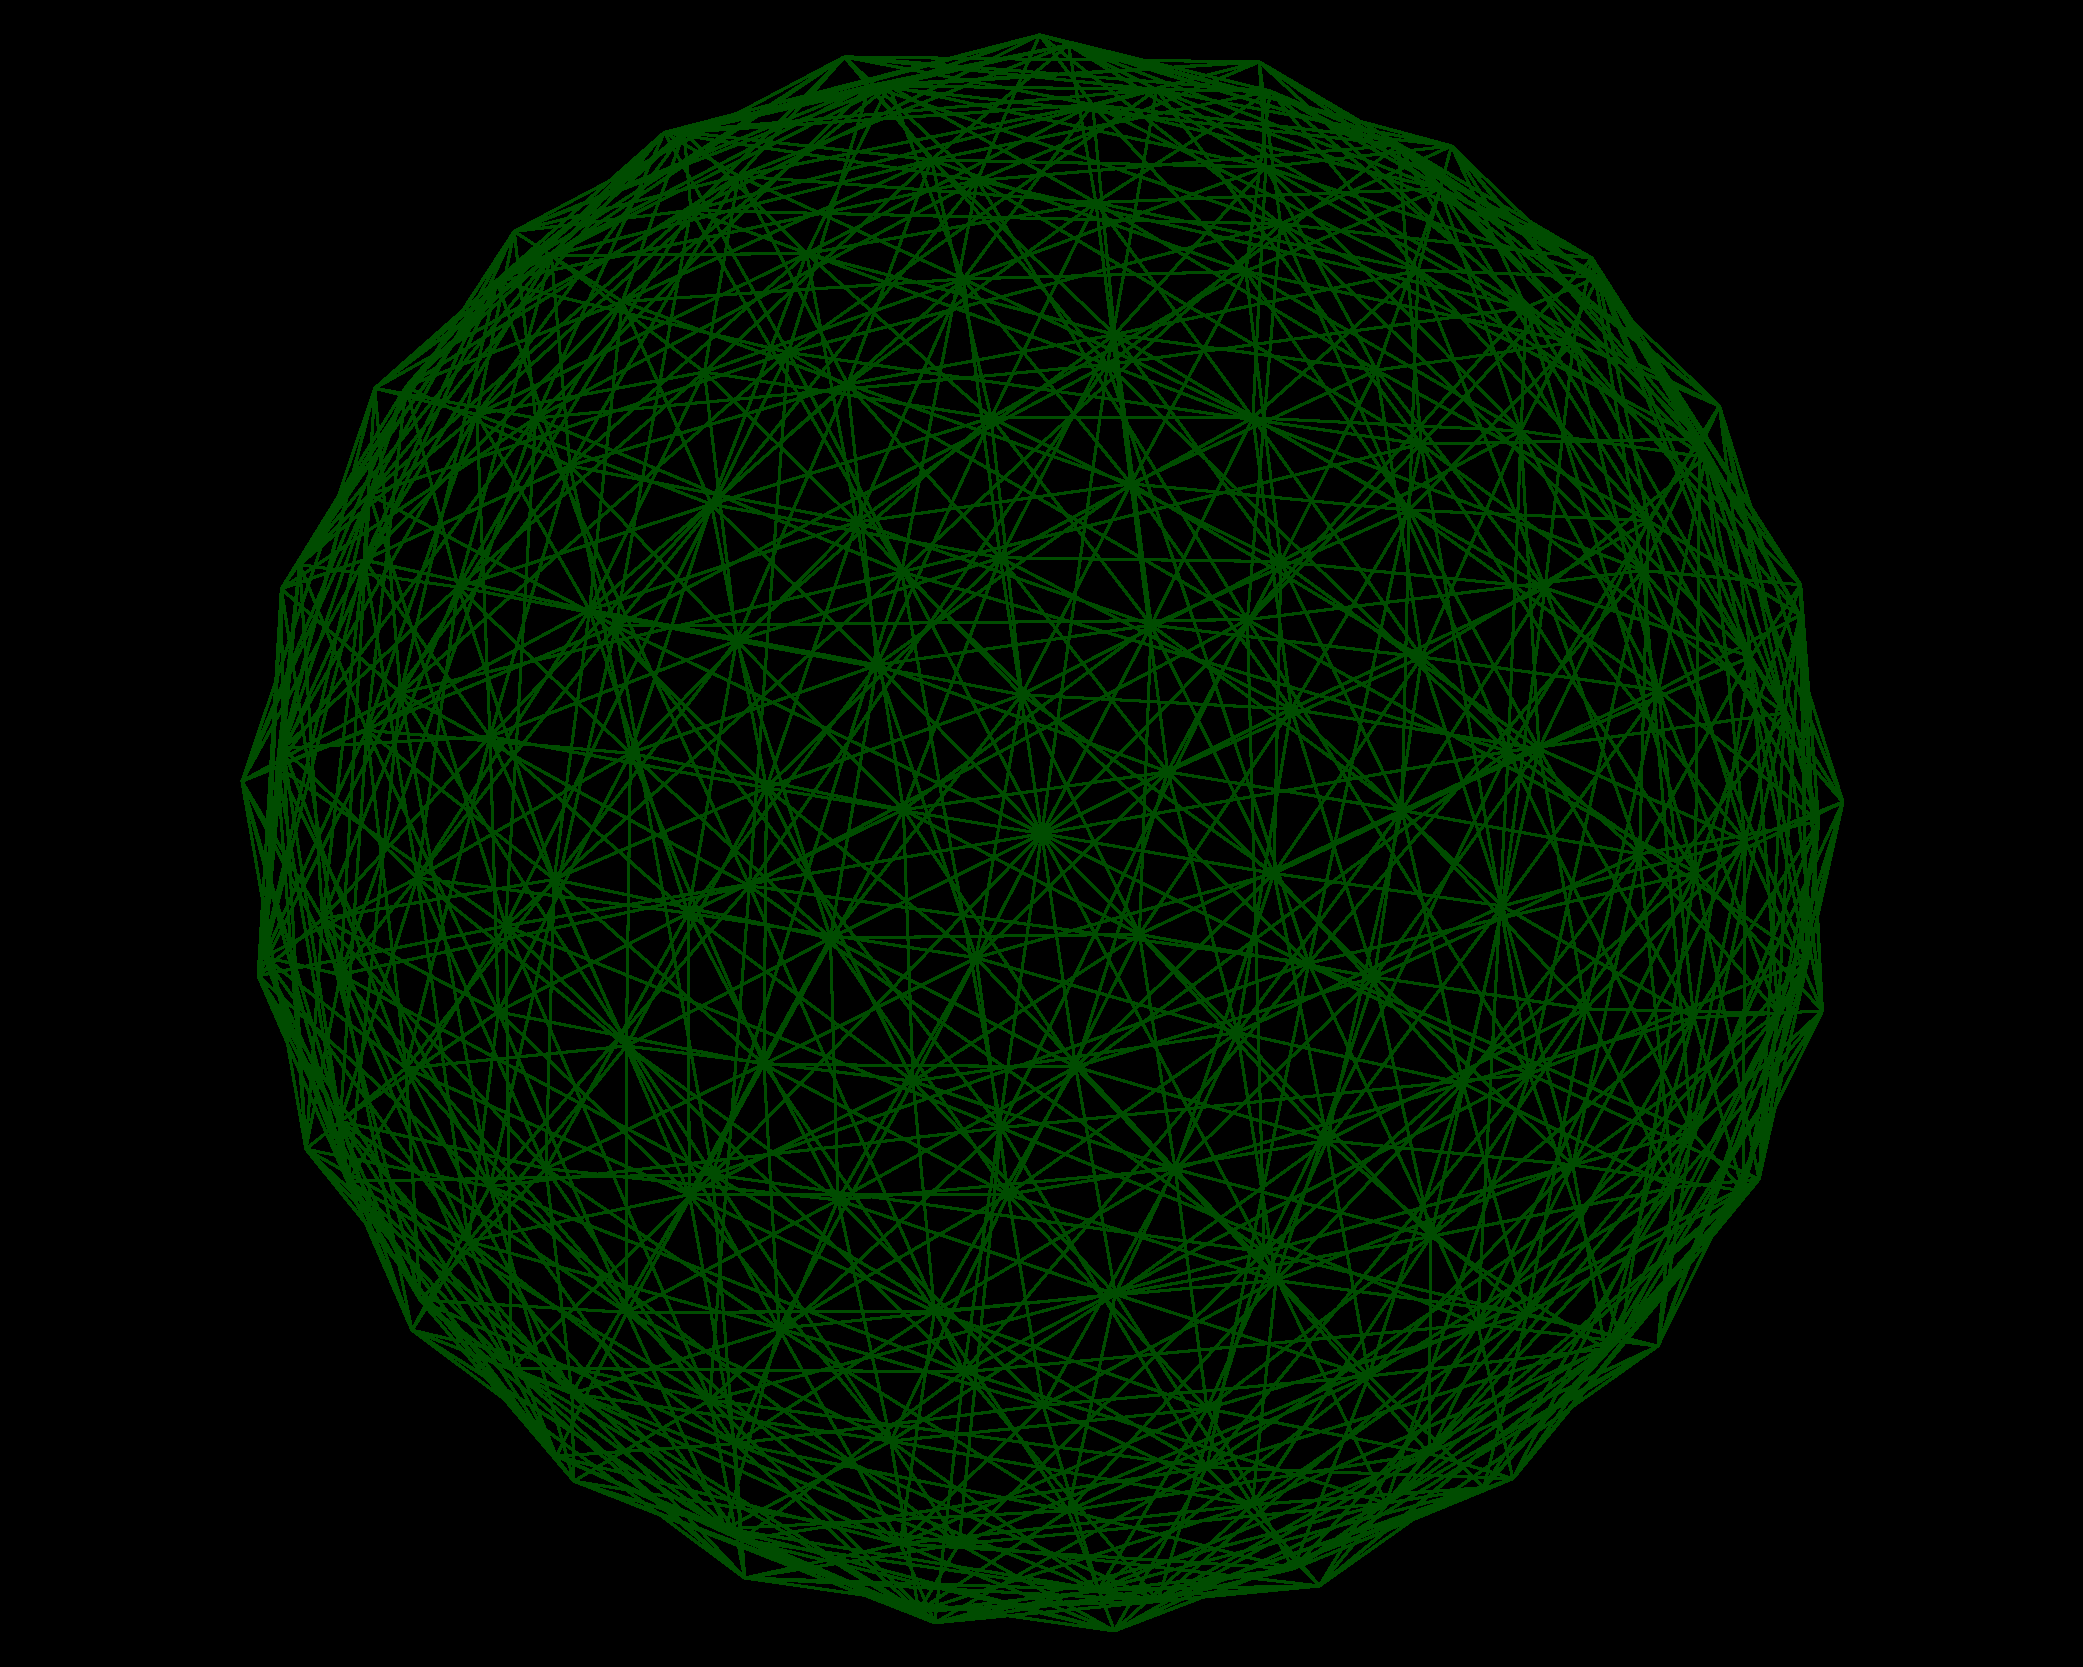
\includegraphics[width=0.37\paperwidth]{chapters/chapter3/program_viz4.pdf}}
%\vspace{1ex}
%\end{minipage}\hfill
%\begin{minipage}[b]{0.5\linewidth}
%\center{\includegraphics[width=0.37\paperwidth]{chapters/chapter3/program_viz3.pdf}}
%\vspace{1ex}
%\end{minipage}\hfill
%\begin{minipage}[b]{0.5\linewidth}
%\center{\includegraphics[width=0.37\paperwidth]{chapters/chapter3/program_viz2.pdf}}
%\vspace{1ex}
%\end{minipage}\hfill
%\begin{minipage}[b]{0.5\linewidth}
%\center{\includegraphics[width=0.37\paperwidth]{chapters/chapter3/program_viz1.pdf}}
%\vspace{1ex}
%\end{minipage}\hfill

\center{\includegraphics[width=0.7\paperwidth]{chapters/chapter3/kek.png}}
\caption{Пример визуализации раскраски.}
\label{chapter3:fig:viz}
\end{figure}

\vspace{5pt}
\textbf{3.2 Теоретические оценки}\label{chapters:3.2}
\vspace{5pt}

\begin{lemma}\label{chapter3:lemma}
Пусть $G$ содержит такую вершину $v$ степени $5$, что каждая из смежных с ней вершин имеет степень $6$. 
Тогда $\chi(G^2) \ge 8$. В частности, при $p,q \ge 1$ выполнено $\chi(T^2) \ge 8$.
\end{lemma}

\begin{figure}[h]
\centering
\captionsetup{justification=centering}
\center{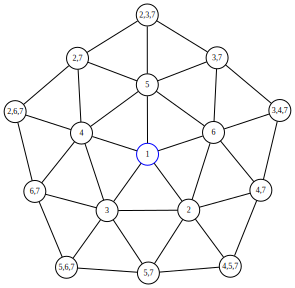
\includegraphics[width=0.45\paperwidth]{chapters/chapter3/cap.pdf}}
\caption{К лемме \ref{chapter3:lemma}.}
\label{chapter3:fig:lemma}
\end{figure}

\begin{proof}
На \figurename{ \ref{chapter3:fig:lemma}} приведены возможные цвета вершин в окрестности вершины степени $5$ (без ограничения общности). 
Тогда из вершин \enquote{внешнего} пояса не более трех имеют цвет $7$, а остальные $7$ вершин раскрашены в цвета $2$--$6$. Но это невозможно, поскольку из этих $7$ вершин можно покрасить в любой из цветов $2$--$6$ не более одной. 
\end{proof}




В заключение приведем основной теоретический результат данной работы.

\begin{theorem}\label{chapter3:theorem}
При $r \geq r_0 = \sqrt{\frac{153^2}{1220}}$ для раскраски областей сферической диаграммы Вороного,
удовлетворяющей условиям \ref{chapter1:eq:diams}, \ref{chapter1:eq:radiuseq}, 
потребуется по крайней мере $8$ цветов.
\end{theorem}

\begin{myproof}
Пусть $T$ -- двойственная триангуляция диаграммы Вороного. 
Предположим, что существует правильная раскраска $T^2$ в $7$ цветов.
Тогда $T$ не содержит вершины  степени $7$ или более (для раскраски ее $1$-окрестности потребуется $8$ цветов).
Поскольку суммарный дефект вершин равен $12$, число вершин в ненулевым дефектом не больше $12$. 
Назовем такие вершины \textit{дефектными}.

Заметим, что раскраска полоски ширины $4$, состоящей из шестиугольников, определяется однозначно конечным участком 
(на \figurename{ \ref{chapter3:fig:hex_determ}} последовательно раскрашиваются шестиугольники $a,\,b,\,c,\,d$). 
Это рассуждение, разумеется, можно сформулировать и в терминах раскрасок $T$.

\begin{figure}[h]
\centering
\captionsetup{justification=centering}
\includegraphics[width=10cm]{chapters/chapter3/hex_determ.png}
\caption{К теореме \ref{chapter3:theorem}.}
\label{chapter3:fig:hex_determ}
\end{figure}

Пусть $T_1$ -- подграф $T$, полученный как объединение всех $4$-окрест\-нос\-тей дефектных вершин; 
$T_2$ -- подграф $T_1$, состоящий из вершин $T_1$, находящихся на расстоянии не более $4$ от некоторой вершины из 
$V(T) \backslash V(T_1)$. Предположим, что $T_2$ непуст. Очевидно, $T_2$ является планарным, как и $T$. 
Любой цикл на этом графе разбивает графы $T, \, T_2$ на две части в смысле укладки на плоскости (сфере) и теоремы Жордана. Обозначим внутреннюю часть $\operatorname{int} L$.

\begin{lemma}
Пусть правильная раскраска $T$ в 7 цветов существует, и $L=(v_1,v_2, \dots , v_l, v_1)$ -- некоторый простой цикл на $T_2$. 
Тогда сумма дефектов вершин $T$ внутри (снаружи) $L$ делится на 6.
\end{lemma}

\begin{myproof}

Рассмотрим допустимую раскраску $T$ (и вершин $L$) в 7 цветов. 
Припишем каждой упорядоченной паре цветов $(i,j)$ направление 
$\phi_{ij}=k\pi/3$, $k \in \{ \, 0, 1, \dots , 5 \, \}$, соответствующее переходу между данной парой в раскраске плоскости. 
Каждой паре соседних вершин $v_s, v_{s+1}$ соответствует некоторое направление $\phi_s$, 
причем при обходе $L$ оно остается неизменным, если эта вершина имеет $2$-x соседей внутри и $2$-x вне $L$, 
иными словами, если к ней внутри и вне $L$ примыкает по $3$ треугольника триангуляции, порожденной вложением $T$ в плоскость. 
Если снаружи $4$ треугольника, а внутри -- $2$, то  $\phi_{s+1}=\phi_s-\pi/3$ и т.~д.:
$$\phi_{s+1}-\phi_{s} = \frac{\pi}{6} \left( \Delta_{in}(v)- \Delta_{out}(v) \right),$$
где $\Delta_{in}(v)$, $\Delta_{out}(v)$ -- число треугольников, примыкающих к вершине, 
соответственно, внутри и снаружи области, ограниченной путем $L$. 

Назовем дефектом пути число

$$\delta(L) = \sum\limits_{s} \frac{1}{2} \left(\Delta_{in}(v_s) - \Delta_{out}(v_s) \right).$$
Для любого замкнутого пути на триангуляции из формулы Эйлера следует, что 

$$\delta(L) = 6 - \sum\limits_{v \, \in \, \operatorname{int} L} \delta(v).$$
Остается заметить, что $$\sum\limits_{s=1}^l \left(\phi(v_{s+1}) - \phi(v_s)\right) = 2\pi k = \frac{\pi}{3} \delta(L),$$ 

$$\delta(L)=6k.$$

\end{myproof}

Продолжая доказательство основной теоремы, рассмотрим два случая.

1. Граф $T_2$ пустой. Тогда каждая $4$-окрестность дефектной вершины содержит не более $1+5+10+15+20=51$ вершины, 
а общее число вершин не превосходит $12 \cdot \frac{51}{2} = 306$. 
Площадь области диаметра $1$ на сфере радиуса $r$ оценивается сферху площадью сферического сегмента
$$S_i \leq S_{max} = 2 \pi r^2 \left(1- \sqrt{1-\frac{1}{4r^2}}\right).$$
Запишем неравенство для площади сферы:

$$ 612 \pi r^2 \left(1- \sqrt{1-\frac{1}{4r^2}}\right) \geq 4 \pi r^2; $$

$$ 1- \sqrt{1-\frac{1}{4r^2}} \geq \frac{1}{153}; $$

$$ \sqrt{1-\frac{1}{4r^2}} \leq \frac{152}{153}; $$

$$ 1-\frac{1}{4r^2} \leq \frac{152^2}{153^2}; $$

$$ \frac{1}{4r^2} \geq 1 - \frac{152^2}{153^2} = \frac{305}{153^2}; $$

$$ 4r^2 \leq \frac{153^2}{305}; $$

$$ r \leq \sqrt{\frac{153^2}{1220}} \approx 4.38. $$

2. Граф $T_2$ непуст. Тогда число вершин в $T$, вообще говоря, не ограничено комбинаторными соображениями, 
но дефектные вершины должны образовывать два подмножества с общим дефектом $6$ в каждом, 
а длина пояса из шестиугольников между этими двумя группами вершин не превосходит $20$, 
и этот пояс покрывает \enquote{экватор} сферы. Следовательно,

$$ 20 r \cdot 2 \arcsin \frac{1}{2 r} \geq 2 \pi r; $$

$$ \arcsin \frac{1}{2 r} \geq \frac{\pi}{20}; $$

$$ \frac{1}{2 r} \geq \sin \frac{\pi}{20}; $$

$$ r < \frac{1}{2 \sin \frac{\pi}{20}} \approx \frac{10}{\pi} \approx 3.18. $$

\end{myproof}

\newpage
\begin{center}
\noindent\textbf{ЗАКЛЮЧЕНИЕ}\label{chapters:conclusions}
\vspace{1.5mm}
\end{center}

В данной работе рассматривалась задача о построении раскрасок двумерных сфер с запрещенными единичными расстояниями. 
В ходе работы были полностью решены все поставленные задачи и получены следующие эмпирические и теоретические результаты:

\begin{enumerate}[leftmargin=1cm,topsep=0pt,itemsep=-1ex,partopsep=1ex,parsep=1ex,label=\arabic{*}.]

\item Установлено, что семейство раскрасок в $8$ и $9$ цветов можно получить на основе сферических диаграмм Вороного, соответствующих локальным минимумам задачи Томсона.  

\item Получены оценки хроматических чисел двойственных графов для регулярных решений задачи Томсона с икосаэдральной симметрией, которые являются квадратами соответствующих графов триангуляций.

\item Получены раскраски и оценки хроматических чисел сфер при некоторых диапазонах значений радиуса.

\item Дан обзор алгоритмов и методов, применяемых при построении современных \textit{SAT}-решателей.

\item Разработан программнай код, конструирующий корректные раскраски двумерной сферы на основе решения задачи Томсона.

\item Разработана программа для визуализации сферических диаграмм Вороного и их раскрасок.

\end{enumerate}

Программный код и все материалы, необходимые для воспроизведения полученных результатов розмещены странице GitHub [30] в открытом доступе.

Несмотря на то, что данная работа является еще одним небольшим шагом к решению задачи о раскраске сфер, полученные результаты нельзя назвать исчерпывающими. Среди открытых вопросов и направлений для дальнейших исследований можно отметить следующие:

\begin{enumerate}[leftmargin=1cm,topsep=0pt,itemsep=-1ex,partopsep=1ex,parsep=1ex,label=\arabic{*}.]

\item Доказательство оценки для хроматического числа квадрата двойственного графа регулярных триангуляций сферы.
\item Доказательство общей оценки хроматического числа сферы для достаточно больших значений радиуса.
\item Постановка и решение аналогичных задач для трехмерных сфер.
\item Изучение случая сферы с радиусом $\frac{1}{2+\epsilon}$.

\end{enumerate}



\newpage
\begin{center}
\noindent\textbf{СПИСОК ИСПОЛЬЗОВАННЫХ ИСТОЧНИКОВ}\label{chapters:biblio}
\vspace{1.5mm}
\end{center}

\begin{enumerate}[leftmargin=0.5cm,topsep=0pt,itemsep=-1ex,partopsep=1ex,parsep=1ex,ref=\arabic{*},label=\arabic{*}.]

\item\label{bib:Cook}
Cook S. A. The complexity of theorem-proving procedures //Proceedings of the third annual ACM symposium on Theory of computing. – 1971. – С. 151-158.

\item\label{bib:Karp}
Karp R. M. Reducibility among combinatorial problems //Complexity of computer computations. – Springer, Boston, MA, 1972. – С. 85-103.

\item\label{bib:Rolf}
Rolf D. Improved bound for the PPSZ/Schöning-algorithm for 3-SAT //Jour\-nal on Satisfiability, Boolean Modeling and Computation. – 2006. – Т. 1. – №. 2. – С. 111-122.

\item\label{bib:Robinson1962}
Robinson J. A. Martin Davis, George Logemann, and Donald Loveland. A machine program for theorem-proving. Communications of the ACM, vol. 5 (1962), pp. 394–397 //The Journal of Symbolic Logic. – 1967. – Т. 32. – №. 1. – С. 118-118.

\item\label{bib:MarquesSilva}
Marques-Silva J., Malik S. Propositional SAT solving //Handbook of Model Checking. – Springer, Cham, 2018. – С. 247-275.

\item\label{bib:Lardeux}
Lardeux F., Saubion F., Hao J. K. GASAT: a genetic local search algorithm for the satisfiability problem //Evolutionary Computation. – 2006. – Т. 14. – №. 2. – С. 223-253.

\item\label{bib:Selsam}
Selsam D. et al. Learning a SAT solver from single-bit supervision //arXiv preprint arXiv:1802.03685. – 2018.

\item\label{bib:HeuleBiere}
Heule M., Biere A. Proofs for satisfiability problems //All about Proofs, Proofs for all. – 2015. – Т. 55. – №. 1. – С. 1-22.

\item\label{bib:HeuleKullmann}
Heule M. J. H., Kullmann O., Marek V. W. Solving and verifying the boolean pythagorean triples problem via cube-and-conquer //International Conference on Theory and Applications of Satisfiability Testing. – Springer, Cham, 2016. – С. 228-245.

\item\label{bib:ZaikinKochemazovSemenov}
Zaikin O., Kochemazov S., Semenov A. SAT-based search for systems of diagonal latin squares in volunteer computing project sat@ home //2016 39th International Convention on Information and Communication Technology, Electronics and Microelectronics (MIPRO). – IEEE, 2016. – С. 277-281.

\item\label{bib:Järvisalo}
Järvisalo M. et al. The international SAT solver competitions //Ai Magazine. – 2012. – Т. 33. – №. 1. – С. 89-92.
	
\item\label{bib:BiereCadical}
Biere A. Cadical, Lingeling, Plingeling, Treengeling and YalSAT entering the sat competition 2018 //Proc. of SAT Competition. – 2018. – С. 13-14.

\item\label{bib:HoosStützle}
Hoos H. H., Stützle T. SATLIB: An online resource for research on SAT //Sat. – 2000. – Т. 2000. – С. 283-292.

\item\label{bib:HoosWalkSAT}
Hoos H. H., Stützle T. Local search algorithms for SAT: An empirical evalua\-ti\-on //Journal of Automated Reasoning. – 2000. – Т. 24. – №. 4. – С. 421-481.

\item\label{bib:Sorensson}
Sorensson N., Een N. Minisat v1. 13-a sat solver with conflict-clause mini\-mi\-za\-ti\-on //SAT. – 2005. – Т. 2005. – №. 53. – С. 1-2.

\item\label{bib:BiereHeule}
Biere A., Heule M., van Maaren H. (ed.). Handbook of satisfiability. – IOS press, 2009. – Т. 185.

\item\label{bib:Puri}
Puri R., Gu J. A BDD SAT solver for satisfiability testing: An industrial case study //Annals of Mathematics and Artificial Intelligence. – 1996. – Т. 17. – №. 2. – С. 315-337.

\item\label{bib:MarquesSilva1999}
Marques-Silva J. The impact of branching heuristics in propositional satisfiabi\-li\-ty algorithms //Portuguese Conference on Artificial Intelligence. – Springer, Berlin, Heidelberg, 1999. – С. 62-74.

\item\label{bib:EénBiere}
Eén N., Biere A. Effective preprocessing in SAT through variable and clause elimination //International conference on theory and applications of satisfiabi\-li\-ty testing. – Springer, Berlin, Heidelberg, 2005. – С. 61-75.

\item\label{bib:Moskewicz}
Moskewicz M. W. et al. Chaff: Engineering an efficient SAT solver //Procee\-dings of the 38th annual Design Automation Conference. – 2001. – С. 530-535.

\item\label{bib:Kullmann2009}
Kullmann O. Theory and applications of satisfiability testing //SAT. – 2009. – С. 147.

\item\label{bib:Katebi}
Katebi H., Sakallah K. A., Marques-Silva J. P. Empirical study of the anatomy of modern sat solvers //International Conference on Theory and Applications of Satisfiability Testing. – Springer, Berlin, Heidelberg, 2011. – С. 343-356.

\item\label{bib:Nadel2002}
Nadel A. Backtrack search algorithms for propositional logic satisfiability: Review and innovations. – Hebrew University of Jerusalem, 2002.

\item\label{bib:Newsham}
Newsham Z. et al. SATGraf: Visualizing the evolution of SAT formula struc\-tu\-re in solvers //International Conference on Theory and Applications of Satisfiabi\-li\-ty Testing. – Springer, Cham, 2015. – С. 62-70.

\item\label{bib:SATzilla}
Xu L. et al. SATzilla: portfolio-based algorithm selection for SAT //Journal of artificial intelligence research. – 2008. – Т. 32. – С. 565-606.

\item\label{bib:Heule2018}
Heule M. J. H. Computing small unit-distance graphs with chromatic number 5 //arXiv preprint arXiv:1805.12181. – 2018.

\item\label{bib:Soifer}
Soifer A. The mathematical coloring book: Mathematics of coloring and the colorful life of its creators. – Springer Science \& Business Media, 2008.

\item\label{bib:Kronk}
Kronk H. V., Mitchem J. A seven-color theorem on the sphere //Discrete Mathematics. – 1973. – Т. 5. – №. 3. – С. 253-260.

\item\label{bib:BruijnErdos}
Bruijn N. G., Erdos P. A colour problem for infinite graphs and a problem in the theory of relations //Indigationes Mathematicae. – 1951. – Т. 13. – С. 371-373.

\item\label{bib:Simmons}
Simmons G. J. The chromatic number of the sphere //Journal of the Austra\-li\-an Mathematical Society. – 1976. – Т. 21. – №. 4. – С. 473-480.

\item\label{bib:RaiSphere}
Raigorodskii A. M. On the chromatic numbers of spheres in $\mathbb{R}^n$ //Combinato\-ri\-ca. – 2012. – Т. 32. – №. 1. – С. 111-123.

\item\label{bib:Nech}
Oren Nechushtan. On the space chromatic number. Discrete mathematics, 256(1):499–507, 2002.

\item\label{bib:Coul}
David Coulson. A 15-colouring of 3-space omitting distance one. Discrete mathematics, 256(1):83–90, 2002.

\item\label{bib:Rai1}
Андрей М. Райгородский. О хроматическом числе пространства. Успехи математических наук, 55(2):147–148, 2000.

\item\label{bib:Larm}
David G. Larman and Ambrose C. Rogers. The realization of distances within sets in Euclidean space. Mathematika, 19(01):1–24, 1972. 

\item\label{bib:Rogers}
Rogers C. A. Covering a sphere with spheres //Mathematika. – 1963. – Т. 10. – №. 2. – С. 157-164.

\item\label{bib:Pros}
Prosanov R. Chromatic numbers of spheres //Discrete Mathematics. – 2018. – Т. 341. – №. 11. – С. 3123-3133.

\item\label{bib:Kostina}
Костина О. А., Райгородский А. М. О новых нижних оценках хроматического числа сферы //Труды Московского физико-технического института. – 2015. – Т. 7. – №. 2 (26).

\item\label{bib:ErdosGraham}
Erdos P., Graham R. L. Problem proposed at the 6th Hungarian combinato\-ri\-al conference //Eger. July. – 1981.

\item\label{bib:Larrea}
Larrea V. G. V. Construction of Delaunay Triangulations on the Sphere: A Parallel Approach. – 2011.

\item\label{bib:Thomson}
Thomson J. J. XXIV. On the structure of the atom: an investigation of the stability and periods of oscillation of a number of corpuscles arranged at equal intervals around the circumference of a circle; with application of the results to the theory of atomic structure //The London, Edinburgh, and Dublin Philosophical Magazine and Journal of Science. – 1904. – Т. 7. – №. 39. – С. 237-265.

\item\label{bib:Katanforoush}
Katanforoush A., Shahshahani M. Distributing points on the sphere, I //Ex\-pe\-ri\-men\-tal Mathematics. – 2003. – Т. 12. – №. 2. – С. 199-209.

\item\label{bib:Altschuler}
Altschuler E. L. et al. Possible global minimum lattice configurations for Thomson's problem of charges on a sphere //Physical Review Letters. – 1997. – Т. 78. – №. 14. – С. 2681.

\item\label{bib:Barber}
Barber C. B., Dobkin D. P., Huhdanpaa H. Qhull: Quickhull algorithm for computing the convex hull //Astrophysics Source Code Library. – 2013.

\item\label{bib:Wales}
Wales D. J. et al. The Cambridge cluster database. – 2001.

\end{enumerate}




\definecolor{codegreen}{rgb}{0,0.6,0}
\definecolor{codegray}{rgb}{0.5,0.5,0.5}
\definecolor{codepurple}{rgb}{0.58,0,0.82}
\definecolor{backcolour}{rgb}{0.95,0.95,0.92}

\lstdefinestyle{mystyle}{    
    keywordstyle=\color{magenta},
    commentstyle=\color{codegreen},
    lineskip=-1ex,
    numberstyle=\tiny\color{codegray},
    stringstyle=\color{codepurple},
    basicstyle=\ttfamily\footnotesize,
    breakatwhitespace=false,         
    breaklines=true,                 
    captionpos=b,                    
    keepspaces=true,                 
    numbers=left,                    
    numbersep=5pt,                  
    showspaces=false,                
    showstringspaces=false,
    showtabs=false,                  
    tabsize=2,
    xleftmargin=0cm
}

\lstset{style=mystyle}


\newpage
\begin{center}
\noindent\textbf{ПРИЛОЖЕНИЕ 1. ДИАПАЗОНЫ ЗНАЧЕНИЙ РАДИУСА ДЛЯ РЕШЕНИЙ ЗАДАЧИ ТОМСОНА}\label{attachments:1}
\vspace{1.5mm}
\end{center}

\begin{longtable}{ccll} 
\hline
n & k & $r_{min}$ & $r_{max}$ \\ 
\hline
\endhead
\input{chapters/attachments/colorings2.txt}
\hline
\end{longtable}

\newpage
\begin{center}
\noindent\textbf{ПРИЛОЖЕНИЕ 2. КОДИРОВАНИЕ ЗАДАЧИ РАСКРАСКИ ГРАФА}\label{attachments:2}
\vspace{1.5mm}
\end{center}

\lstinputlisting[language=Python]{chapters/attachments/g2cnf.py}

\newpage
\begin{center}
\noindent\textbf{ПРИЛОЖЕНИЕ 3. ВЫЧИСЛЕНИЕ ГРАНИЦ ДИАПАЗОНОВ ЗНАЧЕНИЙ РАДИУСА}\label{attachments:3}
\vspace{1.5mm}
\end{center}

\lstinputlisting[language=Python]{chapters/attachments/build_gs.py}

\newpage
\begin{center}
\noindent\textbf{ПРИЛОЖЕНИЕ 4. ПОСТРОЕНИЕ ДИАГРАММЫ ВОРОНОГО С ИКОСАЭДРАЛЬНОЙ СИММЕТРИЕЙ}\label{attachments:4}
\vspace{1.5mm}
\end{center}

\lstinputlisting[language=Python]{chapters/attachments/sphere_triang.py}

\newpage
\begin{center}
\noindent\textbf{ПРИЛОЖЕНИЕ 5. ВИЗУАЛИЗАЦИЯ РАСКРАСОК}\label{attachments:5}
\vspace{1.5mm}
\end{center}

\lstinputlisting[language=C++]{chapters/attachments/Utils.hpp}

\lstinputlisting[language=C++]{chapters/attachments/sphere.cpp}


\end{document}